
\documentclass{article}
\usepackage{appendix}
\usepackage{amsmath}
\usepackage{caption}
\usepackage{placeins}
\usepackage{graphicx}
\usepackage{subcaption}
\usepackage{tikz}
%\usepackage[active,tightpage]{preview}
\usepackage{natbib}
\bibpunct{(}{)}{,}{a}{}{;} 
\usepackage{url}
\usepackage{nth}
% for the d in integrals
\newcommand{\dd}{\; \mathrm{d}}
\newcommand{\ec}{\quad\quad\text{,}}
\newcommand{\ep}{\quad\quad\text{.}}

\usepackage[top=2in, bottom=1.5in, left=1in, right=1in]{geometry}
\usepackage{setspace}
% matrix numbering
\usepackage{trivfloat}
\trivfloat{matrix}
\floatstyle{plaintop}
    \restylefloat{matrix}
\AtBeginDocument{\numberwithin{matrix}{section}}
% end preamble
%-------------------------------------------------------

\begin{document}

\title{Renewal and stability in populations structured by remaining
years of life}
\author{Tim Riffe \\ University of California, Berkeley}
\maketitle

\begin{abstract}
A unisex model of population renewal for populations structured by
thanatological age is presented in both continuous and discrete form. Various
stable and transient properties populations are compared and related when viewed
by chronological versus thanatological age. Results from the two age perspectives are conformable if the starting
population is stable, but are otherwise divergent.
\end{abstract}

*This is a work in progress. All findings are preliminary at this time, so
please don't cite without permission of the author.
\vspace{2em}

\onehalfspacing
All demographic forces vary over age in known and regular ways. Information on
such forces, along with the size and age structure of a population, allows the
demographer to make predictions about the future size and structure of a population. In this
paper, I explore some formal demographic consequences of a particular
redefinition of age. Instead of counting age as the time passed between birth and the present (or
some other moment), consider age as the amount of time left from the present
until death\footnote{This quantity is referred to as \textit{residual} lifetime
in the reliability literaure.}. The first kind of age is called
chronological age and the kind of age explored in this paper is
called thanatological age. Individuals in this case move in the same direction
along imaginary life lines, but the reference point for age is now at the end of the life line instead of at the beginning. For individuals, the timing of events in life is mirrored exactly between the two definitions of age,
but aggregate patterns differ.

Direct information on the timing of demographic transitions with respect to
death is only available from long-running panel or linked historical data that are few and far between. Some surveys also ask respondents in various ways about
their perceived future lifetime, which may underly those
demographic transitions governed to some degree by volition. The present inquiry
draws only from lifetable-projected remaining lifetime, which
is intended to approximate actual remaining lifetime.
The lifetable methods applied here follow those of \citet{brouard1986structure}
or \citet{miller2001increasing}, which redistribute age-classified counts over
future death times according to a fixed mortality schedule. This allows us to make statements about the remaining lifelines within a current stock of population, under certain assumptions.

Temporal perspectives and rescalings of the lifecourse are abundant in
demography already. It is my view that these efforts have enriched the
discipline by producing new insights and questions much more than they have obscured it by
producing conundrums. Likely some demographic phenomena are best
described as a function of time since birth, and others of time until death,
while still others can be a function of both to some degree. Fertility and
reproduction are plausibly a function of both age perspectives, and the question
of how to best partition such forces and events over time is a new conundrum
that I do not tackle here. Instead I describe some of the formal consequences
of the Lotka-Euler renewal model when viewed from the thanatological perspective
of age. The renewal model presented here is not necessarily a suggestion for a
better way to model or project population, but in the minimal sense it
represents an alternative way to tell the story of population renewal.

The chronological-age classified Lotka-Euler renewal model and the
thanatological renewal model both approximate the movement of population stocks
over time, but from opposite vantage points. Specifying a model of thanatological renewal expands the toolbox
available to approach complex temporal population structure. The next section
of this article describes the lifetable method of transforming age-classified
data into thanatological age classes. I then derive the continuous version of
the thanatological renewal model, and some other stable properties. This is
followed by the matrix version of the model, which is explained alongside the
lifecycle graph. I present a set of preliminary empirical findings to help
understand the implications of temporal structure.

\section*{A lifetable approximation of thanatological age}

A lifetable approach to transforming chronologically classified data into
thanatologically classified data is valid when the given lifetable accurately
describes the future mortality of age-classified population. To make
a projective statement about a current stock of population, one does well to
factor in future changes in mortality, and to allow the trajectory of changes
to vary over ages and cohorts. In the case of a stable population model,
mortality is assumed invariant over time, which means that the same survival
pattern underlies each birth cohort. This is the case we explore, and so the
following formulas assume a single lifetable pattern. 

The basic transformation to thanatological age proceeds by defining a
deaths density function, similar the lifetable $d(a)$, but over two
dimensions: chronological age attained, $a$, and remaining years of life, $y$.
This function we denote $d(y|a)$ --- The density distribution of thanatological
age conditional on chronological age. We use the same function name $d()$,
because it is essentially the same notion as the familiar $d(a)$, but rescaled as a
function of chronological age. For ages higher than 0, simply condition
on survival:\footnote{In the reliability literature, our concept of $d(y|a)$ is denoted by \begin{equation} X - t | X > t
\end{equation}
where $X$ is the total lifespan and $t$ is the current chronological age
attained.}

\begin{equation}
\label{eq:vaupel1}
d(y | a) = \mu(a+y)\frac{l(a+y)}{l(a)} \ep
\end{equation}

A convenient discretization of \eqref{eq:vaupel1} is to simply work with the
$d_a$ column of the lifetable (here with single ages):

\begin{equation}
\label{eq:dyadiscret}
d_{y, a} =  \frac{d_{a+y}+d_{a+y+1}}{L_a + L_{a+1}} \ec
\end{equation}

\noindent where $\omega$ is the highest
age.\footnote{Equation~\eqref{eq:dyadiscret} ill incur some error depending on
the method used to derive $L_a$. To remove this error, rescale over the $a$ margin so that each distribution conditioned on $a$
sums to 1. Working with $l_a$ rather than $L_a$ eliminates error and yields
similar results, but is not necessarily better.} One produces in this way a
probability density function over future death times for each chronological age,
$a$. The $d(y|a)$- weighted average of $y$ for a given $a$ returns the familiar
remaining life expectancy column of the lifetable, $e(a)$. If $P(a)$ is a
chronological age-classified population count, we can derive $P(y)$, a
thanatological age-classified population count using

\begin{align}
\label{eq:transform}
P(y) =& \int_0^\infty P(a) d(y | a) \dd a \ep
\end{align}

Since $1 = \int_0^\infty d(y|a) \dd y$ for each $a$,
this density is useful for decomposing data classified by chronological age. For
example, we can break down a population pyramid into thanatological age classes.
Figure~\ref{fig:USdecomp} shows this exercise for 2010 US data, assuming the
2010 period mortality schedule remains constant. When looking from the
chronological age perspective, this decomposition reveals thanatological
heterogeneity, but when viewed from the thanatological perspective
(Figure~\ref{fig:USdecomp}) it reveals chronological age heterogeneity and the
overall thanatological age profile, the future death flow of the current
population.
Figure~\ref{fig:USrecomp} shows this recomposition for the same 2010
US data.

\begin{figure}[ht!]
	\caption{2010 US population structure}
	\begin{center}
	\begin{subfigure}{.45\textwidth}
		\caption{Chronological age-structure (years lived) decomposed by
		thanatological age (years left).}
		\label{fig:USdecomp}
		\includegraphics[scale=.6]{Figures/US2010Age.pdf}
	\end{subfigure}
	~
	\begin{subfigure}{.45\textwidth}
		\caption{Thanatological age-structure (years left) decomposed by chronological
		age (years lived).}
		\label{fig:USrecomp}
		\includegraphics[scale=.6]{Figures/US2010Thano.pdf}
	\end{subfigure}
	\\
	\small{*Population and mortality data from the HMD.}
	\end{center}
\end{figure}

\citet{brouard1986structure} applied this method to highlight regional
differences in French age structure, at times combining this projective method
with historical stocks. \citet{brouard1989mouvements}, and later
\citet{vaupel2009life}, showed that in stationary populations the chronological
and thanatological age structures are identical, and this provides a
limited basis for comparison between the two perspectives. \citet{wachter2014essential} hints at, and
\citet{vaupel2014stable} elaborates on how to make chronological and
thanatological age structure commensurate under a constant growth rate, $r$.
These results will also follow from the following specification of a
thanatological renewal model.

It bears repeating that lifetable-derived thanatological age structure is probabilistic until after death, since it refers to the future according to an assumed mortality pattern.
As such, Figure~\ref{fig:USrecomp} is projective in nature, a forward-looking
glance at population attrition given the population stock and lifetable of a
particular moment, whereas Figure~\ref{fig:USdecomp} is reflective in nature,
since a population's chronological age-structure is mostly the fruit of past
fertility, but also migration and to a lesser degree attrition. Any count
classified by chronological age can be reclassified in this way given a
corresponding lifetable. Exploiting this, we derive thanatological fertility
rates, $f^\star(y)$, by applying \eqref{eq:transform} to age-classified birth
counts, $B(a)$, to get $B(y)$ and again to exposure-to-risk, $E(a)$ (here we
take exposures from all ages), to get $E(y)$ and then dividing

\begin{equation}
f^\star(y) = \frac{B(y}{E(y)} \ep
\end{equation}

We are interested to use thanatological fertility rates, $f^\star(y)$ in
models of population renewal,\footnote{This is probably premature, but helps to
understand the nature and provenance of model components.} rather than to
explicitly study the nature of these rates. Nonetheless it is best not to throw such rates into a model blindly, so we offer a schematic overview of some of their characteristics.
Figure~\ref{fig:FySpaghetti} represents the full variety in
female thanatological period fertility rates that can be found for all years
of data that overlap in the HFD and HMD.\footnote{There are as of this writing
1834 population-years of overlap between the HMD and HFD, including a wide
variety of fertility and mortality combinations.} Figure~\ref{fig:FxSpaghetti} gives ASFR for the same
populations and years as a more familiar reference, but note that both scales
are different. With no indication of particular populations or time series, one
already concludes that period thanatological fertility rates have a
characteristic shape and are not random, erratic or informationless: There is a
pattern to fertility rates by remaining years of life, and it varies over time
and between populations within some range of normality. Thanatological fertility
rates have a wider distribution than do chronological rates. Note that this
spaghetti plot includes both fertility booms and busts, as well as some
mortality crises (1918, WWII). Some patterns to note, but which we do not
separate graphically here, are that the left tail (a gauge of how orphan-prone a
population is) has tended to fall over time. All populations have shown a
rightward shift in both the mean and modal mother's thanatological age at birth
(TAB) over time. Several
populations now show modal TABs of over 60 years. Thanatological total fertility rates (TTFR)
track standard period total fertility rates (PTFR) rather closely, but tend to
be somewhat higher (not shown).

\begin{figure}[h!]
	\caption{Chronological and thantological fertility rates, all 1600
	country-year combinations present in both the HFD and HMD.* Note different x
	and y scales.}
	\label{fig:Fxcompare}
	\begin{center}
	\makebox[\textwidth]{
	\begin{subfigure}{.45\textwidth}
		\caption{Chronological period fertility rates.}
		\label{fig:FxSpaghetti}
		\includegraphics[scale=.45]{Figures/FxSpaghettiDraft.png}
	\end{subfigure}
	~
	\begin{subfigure}{.45\textwidth}
		\caption{Thanatological period fertility rates.}
		\label{fig:FySpaghetti}
		\includegraphics[scale=.45]{Figures/FySpaghettiDraft.png}
	\end{subfigure}
	}
	\\
	\end{center}
	\begin{tiny}
	*AUT, $1951-2010$; BGR, $1947-2009$; BLR, $1964-2009$; CAN, $1921-2007$; 
	CHE, $1932-2011$; CZE, $1950-2011$; DEUTE, $1956-2010$; DEUTNP, $1990-2010$; 
	DEUTW, $1956-2010$; ESP, $1922-2006$; EST, $1959-2010$; FIN, $1939-2009$; 
	FRATNP, $1946-2010$; GBR\_NIR, $1974-2009$; GBR\_NP, $1974-2009$; GBR\_SCO,
	$1945-2009$; GBRTENW, $1938-2009$; HUN, $1950-2009$; IRL, $1955-2009$; JPN, $1947-2009$; 
	LTU, $1959-2010$; NLD, $1950-2009$; NOR, $1967-2009$; PRT, $1940-2009$; 
	RUS, $1959-2010$; SVK, $1950-2009$; SVN, $1983-2009$; SWE, $1891-2010$; 
	TWN, $1976-2010$; UKR, $1959-2006$; USA, $1933-2010$
	\end{tiny}
\end{figure}

In general, thanatological fertility rates will not be useful for purposes of
projection, unless the demographer believes that their empirical regularity is
somehow stronger than typical ASFR. This is a question we do not seek to answer
in the present treatment. There are alternative ways of defining
thanatological fertility rates, for instance by transforming the birth and
population vector from a stable population. As proven in appendix~\ref{app:B},
thanatological fertility rates derived from a stable population imply a certain
symmetry with stable populations from the chronological model. First let us
define the basic model.

\FloatBarrier
\section*{The thanatological renewal model}
For the renewal model that follows, we are most interested in using the kind
of fertility rates shown in Figure~\ref{fig:FySpaghetti}, and we refer to a
closed, unisex population based on female vital rates. Assuming constant vital rates, the
births for the present year are given by 
\begin{align}
B(t) =& \int _0^\infty P(y,t)f^\star(y) \dd y = \int _0^\infty P(a,t)f(a) \dd a
\ec \intertext{where $a$ indexes chronological age, $y$ indexes
thanatological age, $P(a), P(y)$ are population counts, and $f^\star(y), f(a)$ are
exact specific fertility probabilities (rates), which here are best thought of
as the fertility rates of females born to females. The thanatological integral can
be broken down back in terms of chronological age:} =& \int_{y=0}^\infty
\int_{a=0}^\infty f^\star(y)\frac{P(a,t)d(a+y)}{l(a)} \dd a \dd y \ec
\intertext{where $d(a)$ is the continuous lifetable death distribution with
radix of 1, so $d(a)/l(0)$. We can relate the present population to past births
with $P(a,t) = B(t-a)l(a)$:}
\label{eq:ergostep1}
=& \int_{y=0}^\infty \int_{a=0}^\infty f^\star(y) B(t-a)d(a+y)\dd a \dd y \ep 
\intertext{Eventually strong ergodicity will assert itself, and $B(t)$ will
be related to $B(t-a)$ according to a constant factor $e^{ra}$, where $r$ is the familiar
intrinsic rate of growth:}
\label{eq:ergostep2}
=& \int_{y=0}^\infty \int_{a=0}^\infty f^\star(y) B(t)e^{-ra}d(a+y)\dd a \dd y
\ep
\intertext{Divide out $B(t)$ to get back a familiar-looking renewal equation:}
\label{eq:thanoren}
1 =& \int_{y=0}^\infty \int_{a=0}^\infty f^\star(y) d(a+y)e^{-ra}\dd a \dd y
\ep
\end{align}
Now compare this to Lotka's chronological formulation
\begin{align}
\label{eq:lotka}
1 =& \int_{a=0}^\infty f(a)l(a)e^{-ra}\dd a \ec
\intertext{which can be expressed as well as}
  =& \int_{a=0}^\infty \int_{y=0}^\infty f(a)d(a+y)e^{-ra}\dd y \dd a \ec
  \label{eq:lotka2}
\end{align}
and note that \eqref{eq:lotka2} and \eqref{eq:thanoren} are really quite
similar, since $\int _{y=0}^\infty d(a+y)\dd a = l(a)$. For intuition, notice that $l(a)$ is here split
up into pieces of $d(a)$, and imagine a 2D surface of these, where one axis is chronological age and the
other axis is thanatological age. For the chronological case \eqref{eq:lotka},
we multiply chronological age-specific fertility rates, $f(a)$, over the
chronological age margin, and for the thanatological case we multiply
$f^\star(y)$ over the thanatological age margin.

There are gaps in the above line of development, since the jump from
\eqref{eq:ergostep1} to \eqref{eq:ergostep2} (strong ergodicity) is unproven,
although it is rather intuitive, given the much greater density of connections
within the model; persons from nearly any thanatologcal age can produce offspring that can have any other thanatological age.\footnote{I say
\textit{nearly} because the very highest thanatological ages tend to be
composed of pre-menarchical females, so these can be thought of as structural
zeros. I am uncertain if it is a record, but it is certainly an extreme case
useful for illustration: Jeanne Calment, who lived to 122, had a daughter at age
22, which means she was about thanatological age 100
(\url{http://en.wikipedia.org/wiki/Jeanne_Calment}). If the lifetable used to
transform to thanatological closes out at age 110+, as is the case with HMD data, then fertility rates for thantological ages 101-110+ would be structural
zeros.} In
this sense, the smoothing mechanism at play as the population passes through
time must be much stronger than that for chronological age, at least in most
cases.  The mechanisms at play unfold in the same way as those so intuitively
described by \citet{arthur1982ergodic}, and said proof may apply here without
further modification. Later in this paper I note how strong ergodicity is
guaranteed given the properties of the thanatolgical projection matrix. A proof
of the uniqueness of the solution to \eqref{eq:thanoren} is given in
Appendix~\ref{app:A}. A proof that the chronological and thanatological renewal
models must yield the same $r$ if the starting population is already stable is
given in Appendix~\ref{app:B}. A fast-converging iterative method for finding
$r$ from equation~\eqref{eq:thanoren} is given in Appendix~\ref{app:C}

If the thanatolgical fertility rates do not derive from a stable
population, as will typicallybe the case, then the two age perspectives
will, unless by coincidence, yield divergent stable models. There is a strong
parallel here with the case of two-sex age-specific fertility rates. As in the
case of divergence between male and female single-sex models, there will
virtually always be divergence between single-sex models under chronological
versus thanatological age, unless the starting population is stable. Even though the modeled population stocks are in a way commensurable, the rates used here, $f(a)$ versus $f^\star(y)$ are calculated on the basis of differently distributed denominators $E(a)$ versus $E(y)$.


Once one finds $r$ from \eqref{eq:thanoren}, other familiar stable population
parameters can be calculated. For instance, we may calculate the mean
thanatological generation time, $T^\star$:
\begin{equation}
\label{eq:Ty}
 T^\star =  \frac{\int _{y=0}^\infty \int _{a=0}^\infty y e^{-ra} d(a+y)
 f^\star(y) \dd a \dd y}{\int _{y=0}^\infty \int _{a=0}^\infty e^{-ra} d(a+y)
 f^\star(y) \dd a \dd y} \ep
\end{equation}
Literally, this is the mean of the remaining lifespans of new mothers in the
stable population. The net reproduction rate, $R_0$ is related by, e.g.,
\begin{equation}
\label{eq:R0fromTy}
R_0 = e^{r T^\star}
\end{equation}
The birth rate, $b$, is given by
\begin{align}
\label{eq:eybrate}
b =& \frac{1}{\int _{y=0}^\infty \int _{a=0}^\infty e^{-ra} d(a+y) \dd a \dd
y}\ec
\intertext{the denominator of which is the inside of
equation~\eqref{eq:thanoren} less $f^\star(y)$. This simplifies to} =&
\frac{1}{ \int _{a=0}^\infty e^{-ra} l(a) \dd a } \ec
\intertext{which is exactly the same as that valid for
chronological age in the Lotka-Euler setup, except that $r$ here comes from the
thanatological renewal model. If the stable age structure, $c^\star(y)$, is
known, then we may take the sum of hypothetical births over thanatological age:}
=& \int _{y=0}^\infty f^\star(y) c^\star(y) \dd y \ep
\end{align}

The stable thanatological age structure, $c^\star(y)$, is the proportion of the stable population with remaining years to live $y$
\begin{align}
\label{eq:cy}
c^\star(y) =& b \int _{a=0}^\infty e^{-ra} d(a+y) \dd a \ec
\intertext{or, given the stable chronological age structure, $c(a)$, and a
lifetable,} =& \int _{a=0}^\infty c(a)d(y|a) \dd a \label{eq:cyfromca}\\ \notag
\\
           =& \frac{\int _{a=0}^\infty d(a+y)e^{-ra}\dd a}{\int
           _{a=0}^\infty l(a)e^{-ra}\dd a}  \ep
\end{align}

It has previously been shown that when $r = 0$ and $y = a$, that
$c(a)=c^\star(y)$ \citep{brouard1989mouvements, vaupel2009life}, and now we can arrive at the same
conclusion directly by equating the chronological and thanatological renewal equations. For
small non-zero magnitude values of $r$ and survival patterns typical of humans, it is also the
case that $c^\star(y|r)\approx c(a|-r)$. This could make a useful heuristic,
and the relationship is asymptotically exact as $r$ approaches zero, but the
exact relationship is to be found in equation~\eqref{eq:cyfromca}. Further
stable population quantities may be estimated by similarly translating the various common definitions (e.g.,
in the glossary of \citet{coale1972growth}) to the present perspective. We will
focus on the main model rather than on these.

\section*{The thanatological projection matrix}
These descriptions can be made more explicit, and in some ways more tractable,
by hashing out the projection matrix that corresponds to the thanatological renewal model. As with the
chronological age-structured Leslie matrix, the thanatological projection
matrix, $\textbf{Y}$, is square and of dimension $y \times y$, where $y$ is the number
of thanatological age classifications on which the population is structured. 
The matrix contains elements for survival and elements for fertility. Unlike
Leslie matrices, $\textbf{Y}$ is not sparse, but is instead populated primarily
with positive entries greater than zero. In the
following, I illustrate using a 6$\times$6 matrix. 

Mortality occurs in only the population class with zero
remaining years of life. The population of thanatological age 1 in year $t$
moves to 0 in year $t + 1$ and dies in the course of that year. Thus, rather than in the
subdiagonal, survival elements are located in the superdiagonal. All survival
values are 1, since there is no decrement until after living through age 0. The survival component of $\textbf{Y}$ is organized as in
Matrix~\ref{matrix:Ysurv}. To imagine a lifecycle graph, each age decrements by
one through each lower age in successive order until being absorbed by death
after completing thanatological age zero.

\begin{matrix}[h!]
\centering
\caption{Survival component of unisex thanatological projection matrix,
$\textbf{Y}$}
\label{matrix:Ysurv}
$\bordermatrix{{e_y } & 0_t & 1_t & 2_t & 3_t & 4_t & 5_t\cr 
                0_{t+1} & 0    &  1   & 0    & 0    & 0    & 0   \cr
                1_{t+1} & 0    &  0   & 1    & 0    & 0    & 0   \cr 
                2_{t+1} & 0    &  0   & 0    & 1    & 0    & 0   \cr 
                3_{t+1} & 0    &  0   & 0    & 0    & 1    & 0   \cr 
                4_{t+1} & 0    &  0   & 0    & 0    & 0    & 1   \cr
                5_{t+1} & 0    &  0   & 0    & 0    & 0    & 0   }$
\end{matrix}

 Fertility inputs to the matrix are derived from single-sex thanatological
 fertility and the lifetable $d_a$ distribution, where $a$ indexes
 chronological age and is equated to $y$ remaining years of life for members
 just born. It is simpler to imagine $d_a$ in this case as indexing the
 future lifespan distribution of newborns. Fertility in a thanatologically
 structured human population occurs in all but the very highest remaining years classes, which can be thought of as structural zeros for simplicity, as they only contain pre-menarchical females
 that will have very long lives.
 For our $6\times 6$ example, say that fertility is observed in
 thanatological classes 0-4, while the final class has no fertility, where
 $f^\star_y$ indicates the fertility probability for class $y$ in the year $t$
 entering population (in the matrix columns). Each $f^\star_y$ is then
 distributed out over rows according to $d_a$.
 The fertility entry in row $m$ and column $n$ of $\textbf{Y}$ will therefore be
 $f^\star_n \cdot d_m$. One can assume that those dying over the course of year
 $t$ (the first column) are exposed to fertility for half of the year,\footnote{One might be tempted to not allow for fertility at all for females dying in year $t$, but recall that fertility is measured in the moment of
 birth, and not conception.} and so discount the fertility entry
 accordingly.
 Further, infant mortality, $f^\star_y \cdot d_0$, located in the first row, must also be discounted, since part
 of the mortality will occur in the same year $t$ and the rest in year $t + 1$. 
 The first row of fertility must be further discounted by a factor, $\lambda$,
 in order to account for the fact that infant mortality is higher in the lower Lexis 
 triangle than in the upper. Of those infants who die in the first year of life,
 a proportion equal to $\lambda$ do not make it to December \nth{31} of the calendar year in which
 they were born.\footnote{$\lambda$ can be derived directly from death counts
 data classified by Lexis triangles. If the demographer
 does not have information to derive $\lambda$ directly, ad hoc or semidirect
 methods may be used to assign a reasonable proportion, such as 0.9 for
 contemporary low mortality populations.} The fertility component of $\textbf{Y}$ is then composed as in Matrix~\ref{matrix:Yfert}.

\begin{matrix}[h!]
\centering
\caption{Fertility component of unisex thanatological projection matrix,
$\textbf{Y}$}
\label{matrix:Yfert}
$\bordermatrix{
  {e_y } \vspace{.6em}&                0_t  & 1_t  & 2_t  & 3_t  & 4_t  & 5_t\cr 
   0_{t+1} \vspace{.6em}& (1-\lambda) \tfrac{f^\star_0d_0}{2} & (1-\lambda) f^\star_1d_0 & (1-\lambda)
   f^\star_2d_0 & (1-\lambda) f^\star_3d_0 & (1-\lambda) f^\star_4d_0 & 0 \cr 
   1_{t+1} \vspace{.6em}& \tfrac{f^\star_0d_1}{2} & f^\star_1d_1 & f^\star_2d_1 & f^\star_3d_1 & f^\star_4d_1
   & 0   \cr 2_{t+1} \vspace{.6em}& \tfrac{f^\star_0d_2}{2} & f^\star_1d_2 & f^\star_2d_2 & f^\star_3d_2 & f^\star_4d_2
   & 0   \cr 3_{t+1} \vspace{.6em}& \tfrac{f^\star_0d_3}{2} & f^\star_1d_3 & f^\star_2d_3 & f^\star_3d_3 & f^\star_4d_3
   & 0   \cr 4_{t+1} \vspace{.6em}& \tfrac{f^\star_0d_4}{2} & f^\star_1d_4 & f^\star_2d_4 & f^\star_3d_4 & f^\star_4d_4
   & 0   \cr 5_{t+1} \vspace{.6em}& \tfrac{f^\star_0d_5}{2} & f^\star_1d_5 & f^\star_2d_5 & f^\star_3d_5 & f^\star_4d_5
   & 0   }$
\end{matrix}
\FloatBarrier

The survival and fertility components of $\textbf{Y}$ add together elementwise,
thus the full 6$\times$6 matrix is composed as in Matrix~\ref{matrix:Y}.

\begin{matrix}[h!]
\centering
\caption{A full unisex thanatological projection matrix, $\textbf{Y}$} 
\label{matrix:Y}
$\textbf{Y} = \bordermatrix{
  {e_y } \vspace{.6em} & 0_t  & 1_t  & 2_t  & 3_t  & 4_t  & 5_t\cr 
  0_{t+1} \vspace{.6em}&  (1-\lambda) \tfrac{f^\star_0d_0}{2} & (1-\lambda) f^\star_1d_0 + 1 &
  (1-\lambda) f^\star_2d_0 & (1-\lambda) f^\star_3d_0 & (1-\lambda) f^\star_4d_0 & 0 \cr 
    1_{t+1} \vspace{.6em}& \tfrac{f^\star_0d_1}{2} & f^\star_1d_1 & f^\star_2d_1 + 1 & f^\star_3d_1 & f^\star_4d_1 & 0 \cr 
    2_{t+1} \vspace{.6em}& \tfrac{f^\star_0d_2}{2} & f^\star_1d_2 & f^\star_2d_2 & f^\star_3d_2 + 1 & f^\star_4d_2 & 0 \cr 
   3_{t+1} \vspace{.6em}& \tfrac{f^\star_0d_3}{2} & f^\star_1d_3 & f^\star_2d_3 & f^\star_3d_3 & f^\star_4d_3 + 1 & 0 \cr 
   4_{t+1} \vspace{.6em}& \tfrac{f^\star_0d_4}{2} & f^\star_1d_4 & f^\star_2d_4 & f^\star_3d_4 & f^\star_4d_4 & 1 \cr 
   5_{t+1} \vspace{.6em}& \tfrac{f^\star_0d_5}{2} & f^\star_1d_5 & f^\star_2d_5 & f^\star_3d_5 & f^\star_4d_5 & 0 }$
\end{matrix}

Figure~\ref{fig:graph} depicts the projection matrix $\textbf{Y}$ in the form of
a lifecycle graph.  In this graph, each thanatological age is a node, and death
is the absorbing state, denoted with an ``X''.
Population members are born into any of the thanatological age classes, and then follow
clockwise around the graph on the thick blue paths in order until finally being
absorbed into death (the node labeled ``X'', not included in the projection matrix). The light gray paths represent fertility. Thse originate from any age class that has a fertility rate greater
than zero, which for this toy matrix are all age classes except the \nth{5}
(highest). The y$^{th}$ age class is subject to the fertility rate $f^\star
(y)$, and these births distribute out to all other age classes according to the
lifespan distribution from the lifetable, $d_a$. Hence, the rate instensity of a
fertility path is determined by the fertility rate of the origin age and
probability of having a lifespan equal to the order of the destination node.  A fraction of
the fertility destined for infant mortality equal to $\lambda$ leads straight to the absorbing state of death. Fertility paths from the \nth{4} thanatological age class have been highlighted. These correspond to the fifth column of the example matrix $\textbf{Y}$, plus an additional path
direct to death for the fraction of infant mortality prior to December \nth{31}
in year $t$. Paths that loop back into the same age class simply indicate those
offspring that are destined to die in the same year as their mother. It is
perhaps clearer to see from the density of this graph and by recalling that
thanatological fertility distributions are relatively wide (see
Figure~\ref{fig:FySpaghetti}) that there is a high degree of mixing of
thanatological age within populations via reproduction -- a strong tendency
toward stability.

\begin{figure}
\centering
\caption{The thanatological lifecycle graph}
\label{fig:graph}
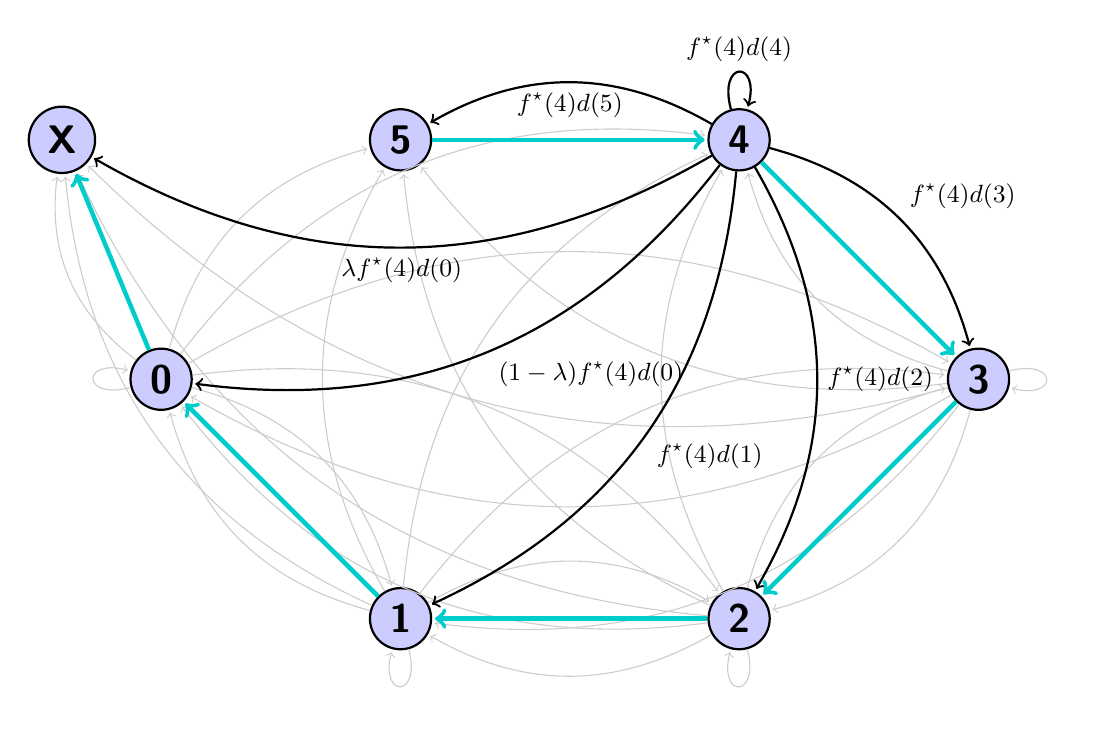
\begin{tikzpicture}[->,shorten >=1pt,auto,node distance=4.3cm,
  thick,main node/.style={circle,fill=blue!20,draw,font=\sffamily\Large\bfseries}]
  \definecolor{gray}{rgb}{0.8,0.8,0.8}
  \definecolor{lightgreen}{rgb}{0,0.8,0.8}
  \node[main node] (0) {0};
  \node[main node] (5) [above right of=0] {5};
  \node[main node] (4) [right of=5] {4};
  \node[main node] (3) [below right of=4] {3};
  \node[main node] (2) [below left of=3] {2};
  \node[main node] (1) [left of=2] {1};
  \node[main node] (X) [left of = 5] {X};

  \path[every node/.style={font=\sffamily\small},draw=gray,thin]
    (3) edge [bend left] node {} (5)
        edge [bend left] node {} (4)
        edge [bend left] node {} (2)
        edge [bend left] node {} (1)
        edge [bend left] node {} (0)  
        edge [bend left] node {} (X)
        edge [loop right] node {} (3) 
    (2) edge [bend left] node {} (5)
        edge [bend left] node {} (4)
        edge [bend left] node {} (3)
        edge [bend left] node {} (1)
        edge [bend left] node {} (0)     
        edge [loop below] node {} (2) 
        edge [bend left] node {} (X)
    (1) edge [bend left] node {} (5)
        edge [bend left] node {} (4)
        edge [bend left] node {} (3)
        edge [bend left] node {} (2)
        edge [bend left] node {} (0)    
        edge [loop below] node {} (1) 
        edge [bend left] node {} (X)
    (0) edge [bend left] node {} (5)
        edge [bend left] node {} (4)
        edge [bend left] node {} (3)
        edge [bend left] node {} (2)
        edge [bend left] node {} (1)
        edge [loop left] node {} (0) 
        edge [bend left] node {} (X);
        
    \path[every node/.style={font=\sffamily\small}]
    (4) edge [bend right] node {$f^\star (4)d(5)$} (5)
        edge [bend left] node {$f^\star (4)d(3)$} (3)
        edge [bend left] node {$f^\star (4)d(2)$} (2)
        edge [bend left] node {$f^\star (4)d(1)$} (1)
        edge [bend left] node {$(1-\lambda)f^\star (4)d(0)$} (0)
        edge [loop above] node {$f^\star (4)d(4)$} (4)
        edge [bend left] node {$\lambda f^\star (4)d(0)$} (X);
    
    \path[every node/.style={font=\sffamily\small}, ultra thick, color =
    lightgreen ] (5) edge node {} (4)
    (4) edge node {} (3)
    (3) edge node {} (2)
    (2) edge node {} (1)
    (1) edge node {} (0)
    (0) edge node {} (X);
        
\end{tikzpicture}
\end{figure}

Thanatological age-classes will ideally terminate at the highest value permitted
by data. For the data used in this paper, there are 111 total age classes, which
translate to 111 total remaining-years classes (0-110+). In practice $\textbf{Y}$ becomes
a 111$\times$111 matrix, with most entries non-zero (nearly complete
connectivity, such as in Figure~\ref{fig:graph}). Construction may appear tedious for
this reason. However, note that the bulk of fertility entries can be derived as the outer (tensor) product $d_a \otimes f_y$, leaving only the first row and first column mortality discounting followed by the addition of the
survival superdiagonal. In most statistical programming languages constructing $\textbf{Y}$ entails only
a couple more lines of code than constructing a Leslie matrix.

Thanatological projection matrices may be manipulated using
standard matrix techniques applicable to the Leslie matrix. Where $\textbf{p}$
is a population vector classified by thanatological age, projection proceeds by
multiplying $\textbf{Y}$ from the left:
$\textbf{p}(t + 1) = \textbf{Y}\textbf{p}(t)$. 

For rate schedules typical of human populations, thanatological projection
matrices are filled with non-negative values, mostly greater than zero. Raising
the matrix to some not-very-large power, $k$, will make all entries greater than zero. This observation, or else by noting that the
lifecylce graph is strongly connected, lets us conclude that the matrix is
irreducible and primitive. By the Perron-Frobenius theorem, the matrix will
 always have a unique, dominant, positive real eigenvalue, the natural
log of which is the intrinsic growth rate, $r$, and strong ergodicity is
assured.
In other words, given a fixed matrix and enough time, the population will conform to some stable thanatological age distribution. Strong
ergodicity was taken for granted in jumping from equation~\eqref{eq:ergostep1}
to ~\eqref{eq:ergostep2}, but the presently described properties of the matrix
model should, albeit unrigorously, satisfy lingering uncertainty on that step.
The eigenvector corresponding to the dominant eigenvalue gives this stable
thanatological age structure. If the fertility rates placed in the matrix are
from the stable population, then the growth rate from the thanatological
projection matrix is equal to that of the standard Leslie
matrix.\footnote{Some care needs to be taken in order to demonstrate this
point, since common approximations and adjustments used in matrix
construction can throw things off. \texttt{R} code is available from the
author to demonstrate this point. See also Appendix~\ref{app:B} for the
corresponding proof from the continuous model.} The square of the, or the pace
of convergence to stability (the ratio of the \nth{1} to the \nth{2} eigenvalues).
\footnote{See \citet[p.86-87]{caswell2001matrix}.}

\section*{Some preliminary empirical findings}
The thanatological renewal equation and the discrete projection matrix can be
put to work with data. In this case a few options are available for determining
what kind of thanatological fertility rates to use. The two obvious choices are
to derive rates from the stable population implied by the chronological renewal
model, or to derive rates such as those from Figure~\ref{fig:FySpaghetti},
based on a particular stock of population. 

Of the 1834 population-years of data on hand, we optimize $r$ from both
\eqref{eq:thanoren} and \eqref{eq:lotka}. In this sample, both versions of $r$
are only plausibly equal in a single instance. Usually thanatological $r$ is
greater than Lotka's $r$ (1373 cases). When Lotka's $r$ is positive (693 cases), thanatological $r$ is greater just over of 50\% of the time (356), but when Lotka's $r$ is negative,
thanatological $r$ is the greater of the two around 90\% of the time (1017
cases). These two approximations of $r$ are of opposite sign 138 times. We
provide a comparison of the $r$ distributions in Figure~\ref{fig:rDist}. Mean
locations for each distribution are indicated with vertical dashed lines; thano.
-0.0010; chrono. -0.0027. The distribution of thanatological $r$ is more compact
than for chronological $r$, with the ratio of variances (thano./chrono.) of
about 0.75. The two theoretical values of $r$ covary strongly, but
thanatological $r$ is the less erratic of the two, and it usually paints a less dire picture when both are negative.

\begin{figure}[h!]
	\caption{Distribution of $r$, chronological (Lotka) and thanatological*.}
	\begin{center}
		\label{fig:rDist}
		\includegraphics[scale=.7]{Figures/rDist.pdf}
	\end{center}
	\begin{tiny}
     * Data from HMD and HFD. Countries and years listed in
     Figure~\ref{fig:Fxcompare}.
	\end{tiny}
\end{figure}

The differences described here are not due primarily to rounding errors in the
data, but rather to the way in which $f^\star(y)$ has been calculated. 
Specifically, in this case we have transformed fertility rates from empirical data with a particular
chronological age structure. If the chronological age structure is far from its
stable distribution, then it may be hard to imagine that $f^\star(y)$ will
remain fixed over time. When holding chronological-age classified fertility rates
fixed, the assumption is just the opposite.

From the projection matrix, the ratio of the largest to the second largest
eigenvalue, the damping ratio, is an indicator of the \textit{springiness} of
the stable population structure, $c^\star(y)$ or $c(a)$, with respect to
disturbances from the stable state as determined by vital rate distributions. A
higher damping ratio means that the population structure oscillates back to
its stable state faster, i.e., that oscillations decrease in size more rapidly. The thanatological damping ratio was
greater than the Leslie damping ratio for all 1834 population-years included in
our empirical analysis. Leslie damping ratios ranged from 1.01258 to 1.0518,
while thanatological damping ratios ranged from 1.0455 to 1.0868. Again, this
was for the raw data, and I am not sure whether this consistent finding is a
natural property of the model or an artifact of the unstable starting state of
the data used to derive thanatological fertility rates. Intuitively, the
thanatological smoothing process should be an order of magnitude stronger than
the chronological smoothing process because each thanatological age class
(node) -- except for the oldest-old -- is connected directly to each other
thanatological age class in both directions. Again, I think contrived examples
will be necessary to shed more light on this finding.

\section{Discussion}
The thanatological renewal model is valid, but this perspective may take some
time to gestate before accepting that it is also a sound description of how
populations renew. What should one imagine under the model of thanatological
population renewal? A useful mnemonic bases itself on Figures~\ref{fig:USdecomp}
and \ref{fig:USrecomp}. In the chronological age-structured model, new
generations appear at the bottom of the pyramid, and move up one rung per year.
All age-classes are subject to attrition, which is spread out over ages and not
readily visible in the pyramid. In the thanatological \textit{leaf}, each birth cohort increments to the population over the whole range of thanatological age
according to $d(a)$, as seen in \eqref{eq:thanoren}, becoming the
shaded layers seen in Figure~\ref{fig:USrecomp}. Each horizontal step is a death
cohort, and these move one step down the pyramid each year without any decrement
(indeed incrementing due to births) until reaching the very bottom. In short,
the locations of increment and decrement, and the direction of movement (when
so visualized) are all switched. The chronological and thanatological renewal
models are almost perfectly opposite descriptions of the same process. 

\vspace{2em}

\begin{appendices}
\section{Unique solution for thanatological $r$}
\label{app:A}
This appendix contains a brief proof that the real solution for the
intrinsic growth rate, $r$, is unique for the case of the thanatological renewal model, \eqref{eq:thanoren}, and can be proven so in
essentially the same fashion as those in existence for the Lotka-Euler model,
\eqref{eq:lotka}. This proof follows that given in
\citet{pressat1973analyse}. Define a convenience function, $I(r)$, for the
integrand of \eqref{eq:thanoren} for a given $r$ and fixed $f^\star(y)$ and $d(a)$:

\begin{equation}
I(r) = \int_{y=0}^\infty \int_{a=0}^\infty f^\star(y) d(a+y)e^{-ra}\dd a \dd y
\end{equation}
Since the death distribution function, $d(a)$, and fertility
function, $f^\star(y)$, are continuous and non-negative, $\lim_{r \to +\infty} I(r)
= 0$ and $\lim_{r \to -\infty} I(r)= \infty$. If $r_2 > r_1$, then $I(r_1) >
I(r_2)$. $I()$ is therefore a continuous and monotonically decreasing function
of $r$ with boundaries that include the value 1 of \eqref{eq:thanoren}, and
 necessarily only obtain this value once. As with the Lotka-Euler equation, there will be more complex
 conjugate solutions for $r$ in the thanatological model,
 and these are not explored in this paper.


\section{Equivalence in stability}
\label{app:B}
This appendix contains a proof that the thanatological renewal equation implies
the same intrinsic growth rate, $r$, as the Lotka-Euler model if
the starting population is stable, given a particular set of thanatological
fertility rates.
This is identical to claiming that the right side of the rewal equation is equal given the same $r$. Since there is a unique
real solution, demonstrated in the previous appendix, then it is sufficient to
show that the two integral equations are equal under these conditions. The basic
relationship is:
\begin{align}
\int _{a=0}^\infty l(a)e^{-ra}f(a) \dd a &= \int _{y=0}^\infty \int
_{a=0}^\infty d(a+y)e^{-ra}f^\star (y) \dd a \dd y
\intertext{when}
f^\star(y) &= \frac{b^\star(y)}{c^\star(y)} \\
b^\star (y) &= \int_{a=0}^\infty b(a) \mu(a+y)\frac{l(a+y)}{l(a)} \dd a \\
c^\star (y) &= \int_{a=0}^\infty c(a) \mu(a+y)\frac{l(a+y)}{l(a)} \dd a
\intertext{Note that:}
c(a) &= \frac{l(a)e^{-ra}}{\int l(a) e^{-ra} \dd a} \\
b(a) &= f(a)c(a)
\end{align}Replacing $f^\star (y)$ with the full expanded
expression and plugging into the thanatological renewal equation gives:
\begin{align}
=& \int _{y=0}^\infty \int
_{a=0}^\infty d(a+y)e^{-ra} \frac{\frac{\int_{t=0}^\infty
f(t)l(t)e^{-rt}\mu(a+y)\frac{l(t+y)}{l(t)} \dd t}{\int l(t) e^{-rt} \dd
t}}{\frac{\int_{t=0}^\infty l(t)e^{-rt} \mu(t+y)\frac{l(t+y)}{l(t)} \dd t}{\int
l(t) e^{-rt} \dd t}} \dd a \dd y
\intertext{The denominator of $c(a)$ cancels out:}
=& \int _{y=0}^\infty \int
_{a=0}^\infty d(a+y)e^{-ra} \frac{
\int_{t=0}^\infty
f(t)l(t)e^{-rt}\mu(t+y)\frac{l(t+y)}{l(t)} \dd t}{
\int_{t=0}^\infty l(t)e^{-rt} \mu(t+y)\frac{l(t+y)}{l(t)} \dd t} \dd a \dd y
\intertext{Some $l(a)$'s also cancel out:}
=& \int _{y=0}^\infty \int
_{a=0}^\infty d(a+y)e^{-ra} \frac{
\int_{t=0}^\infty
f(t)e^{-rt}\mu(t+y)l(t+y) \dd t}{
\int_{t=0}^\infty e^{-rt} \mu(t+y)l(t+y) \dd t} \dd a \dd y
\intertext{Now $d(a+y) = \mu (a+y)l(a+y)$, so we can cancel the inner integral
with the denominator:}
=& \int _{y=0}^\infty 
\int_{a=0}^\infty
f(a)e^{-ra}\mu(a+y)l(a+y) \dd a \dd y
\intertext{Note also that $l(a) = \int _{=a}^\infty d(x) \dd x$ (present
livings are future deaths), which brings us back to the chronological
formulation:} =& \int_{a=0}^\infty e^{-ra}l(a)f(a)
\dd a
\end{align}
This finding essentially proves that in the stable population there is at least
one thanatological fertility rate schedule that will satisfy the constraints of
the lifespan distribution and $r$. However, it is not necessary to derive the
thanatological fertility distribution in the way prescribed here, and indeed an
infinite number of such fertility distributions would satisfy the same
constraints. Imagine these fertility rates cross-classified in
both age dimensions, where two marginal sums give the thanatological and
chronological rates, as they would be calculated over the
corresponding cross-classified exposures. The shape of this rate surface can be
shifted around in infinitely many ways that would preserve a given growth rate
and lifespan distribution, and the above proof shows one such mapping.

\section{An iterative method to find the thanatological $r$}
\label{app:C}
\citet{coale1957new} proposed a fast-converging iterative approach to estimate
the intrinsic growth rate for the Lotka-Euler equation. For the thanatological
renewal model, a similar approach may be taken, with some slight
modifications to Coale's original.
The following steps can be followed to estimate $r$ from
Equation~\eqref{eq:thanoren}:

\begin{enumerate}
  \item Derive a first rough estimate of the mean remaining years of life at
  reproduction, $\widehat{T^\star}$, akin to Lotka's mean generation time, $T$.
  To start, a good-enough guess is to just assume $r=0$:
\begin{equation}
\widehat{T^\star} = \frac{\int _{y=0}^\infty \int _{a=0}^\infty y d (a+y)
f^\star(y) \dd a \dd y}{\int _{y=0}^\infty \int _{a=0}^\infty d(a+y) f^\star(y)
\dd a \dd y}
\end{equation}
  \item A first rough guess at the net reproduction rate, $R_0$ is given by
 \begin{equation}
  R_0 = \int _{y=0}^\infty \int _{a=0}^\infty d(a+y) f^\star(y) \dd a
\dd y
\end{equation}
  \item A first rough estimate of $r$, $r^0$, is given by
   \begin{equation}
   r^0 = \frac{ln(R_0)}{\widehat{T^\star}}
   \end{equation}
  \item Plug $r^0$ into Equation~\eqref{eq:thanoren} to calculate a
  residual, $\delta^0$.
  \item Use $\delta^0$ and $\widehat{T^\star}$ to calibrate the estimate of $r$
  using
  \begin{equation}
  r^{1} = r^0 + \frac{\delta^0}{\widehat{T^\star} - \frac{\delta^0}{r^0}}
  \end{equation}
  \item Repeat step (4) to to derive a new $\delta^i$, then step (5) to refine
  $r^i$, until converging on a stable $r$ after some 20 or so iterations,
  depending on the degree of precision desired ($\widehat{T^\star}$ is not updated
  in this process).
\end{enumerate}

The above procedure is more computationally efficient than minimizing the
absolute residual of Equation~\eqref{eq:thanoren} using a generic
optimizer. Alternatively, one could use the method of cumulants to estimate $r$,
bbut this would entail less precision than the above (unless one goes beyond,
say, five cumulants), and this has not yet been worked out at this time.
 
\end{appendices}
\nocite{HMD,HFD}
-------------------------
% bibliography
\bibliographystyle{plainnat}
  \bibliography{References}  

\end{document}
